% -*- mode: LaTeX; coding: utf-8 -*-
% Typeset with: XeLaTeX

\documentclass[a4paper,11pt]{article}
\usepackage{a4wide}

% Greek fonts
\RequirePackage{fontspec}
\defaultfontfeatures{Ligatures=TeX}
% you may want to try: {Liberation Serif} or {Times New Roman}
\setmainfont{FreeSerif}
% you may want to try: {Liberation Sans} or {Arial}
\setsansfont[Scale=MatchLowercase]{FreeSans}
% you may want to try: {FreeMono} or {Courier New}
\setmonofont[Scale=MatchLowercase]{FreeMono}

\usepackage{mathtools}
\usepackage{tikz}
\usetikzlibrary{positioning}
\usepackage{blkarray}

\newcommand{\indeq}[1]{\stackrel{\text{#1}}{=}}
% Commands for wrapping properly common expressions.
\newcommand{\Exp}{\mathrm{Exp}}
\newcommand{\Expect}{{\rm I\kern-.3em E}}
\newcommand{\Var}{\mathrm{Var}}
\newcommand{\Cov}{\mathrm{Cov}}
\newcommand{\mc}{Μ.Α.Σ.Χ. }

% Main document
\begin{document}
\title{Στοχαστικές Ανελίξεις - 3ο πακέτο Ασκήσεων}
\author{Θωμάς Παππάς}
\date{}
\maketitle

\section*{Άσκηση 1}

Η $\{X(t),t\geq 0\}$ είναι \mc με χώρο καταστάσεων $S = \{0,1,2,\dots\}$.
Τώρα $\forall i \in S$ έχουμε ότι $q_{i,i+1} = \lambda$ (άφιξη πελάτη), ενώ για $i \geq 1$ για τα $q_{i,i-1}$ έχουμε
\begin{itemize}
	\item αν $i=1$ τότε εξυπηρετείτε ένας πελάτης ο οποίος θα εξυπηρετηθεί με ρυθμό $q_{1,0}=\mu$
	\item αν $i \geq 2$ τότε είτε θα τελειώσει η εξυπηρέτηση ενός πελάτη με ρυθμό $\mu$ είτε θα τελειώσει η υπομονή ενός τυχαίου πελάτη στο χώρο αναμονής με ρυθμό $\theta$, δηλαδή
	\[p_{i,i-1} \sim min\{\Exp(\mu), \Exp(\theta)\} = \Exp(\mu+\theta)\]
	και άρα $q_{i,i-1}=\mu+\theta$
\end{itemize}
\begin{center}
	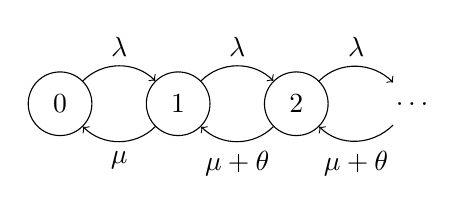
\begin{tikzpicture}[
			node distance={15mm},
			main/.style = {draw, circle, minimum size=23pt},
			dots/.style = {minimum size=15pt}
		]
		\node[main] (1) {$0$};
		\node[main] (2) [right of=1] {$1$};
		\node[main] (3) [right of=2] {$2$};
		\node[dots] (4) [right of=3] {$\dots$};
		\draw[->] (1) to [out=45, in=135] node[above] {$\lambda$} (2);
		\draw[->] (2) to [out=225, in=315] node[below] {$\mu$} (1);
		\draw[->] (2) to [out=45, in=135] node[above] {$\lambda$} (3);
		\draw[->] (3) to [out=225, in=315] node[below] {$\mu+\theta$} (2);
		\draw[->] (3) to [out=45, in=135] node[above] {$\lambda$} (4);
		\draw[->] (4) to [out=225, in=315] node[below] {$\mu+\theta$} (3);
	\end{tikzpicture}
\end{center}
Στη συνέχεια για να βρούμε τη στάσιμη κατανομή θα πάρουμε $\forall j \in S\setminus \{0\}$ το\\
$A_j = \{0,1,2,\dots,j-1\}$ και από τις εξισώσεις γενικευμένης ισορροπίας έχουμε
\begin{itemize}
	\item για $j=1$: $p_0 \cdot q_{01} = p_1 \cdot q_{10} \Rightarrow p_0 \lambda = p_1 \mu \Rightarrow p_1 = \frac{\lambda}{\mu} p_0$
	\item για $j>1$: $p_{j-1} \cdot q_{j-1,j} = p_j \cdot q_{j,j-1} \Rightarrow p_{j-1} \lambda = p_j (\mu+\theta) \Rightarrow p_j = \frac{\lambda}{\mu+\theta} p_{j-1}$
\end{itemize}
Για το τελευταίο βλέπουμε ότι
\[
	p_j = \frac{\lambda}{\mu+\theta} p_{j-1} = \left(\frac{\lambda}{\mu+\theta}\right)^2 p_{j-2} = \cdots = \left(\frac{\lambda}{\mu+\theta}\right)^{j-1} p_1 = \left(\frac{\lambda}{\mu+\theta}\right)^{j-1} \frac{\lambda}{\mu} p_0
\]
Από εξίσωση κανονικοποίησης τώρα έχουμε ότι
\begin{equation}
	\label{eqreg1}
	\sum_{j=0}^\infty p_j = 1 \Rightarrow p_0 + p_1 + \sum_{j=2}^\infty p_j = 1 \Rightarrow p_0 \left(1 + \frac{\lambda}{\mu} + \sum_{j=2}^\infty \left(\frac{\lambda}{\mu+\theta}\right)^{j-1} \frac{\lambda}{\mu} \right) = 1
\end{equation}
Θέτουμε $r = \lambda/(\mu+\theta)$ και υπολογίζουμε το άθροισμα για $r<1$.
\[
	\sum_{j=2}^\infty r^{j-1} \stackrel{k=j-2}{=}  \sum_{k=0}^\infty r^{k+1} = r \sum_{k=0}^\infty r^k = r \left(\frac{1}{1-r}\right) = \frac{\lambda}{\mu+\theta} \cdot \frac{\mu+\theta}{\mu+\theta-\lambda} = \frac{\lambda}{\mu+\theta-\lambda}
\]
Οπότε συνεχίζοντας
\[
	\eqref{eqreg1} \Rightarrow p_0 \left(1 + \frac{\lambda}{\mu} + \frac{\lambda}{\mu} \cdot \frac{\lambda}{\mu+\theta-\lambda} \right) = 1
\]
Θέτουμε $B^{-1} = 1 + \frac{\lambda}{\mu} + \frac{\lambda}{\mu} \cdot \frac{\lambda}{\mu+\theta-\lambda}$ και βλέπουμε ότι $B^{-1} > 0$ οπότε και παίρνουμε
\[p_0 = B\]
Άρα η $\{X(t),t\geq 0\}$ είναι θετικά επαναληπτική αν και μόνον αν $\frac{\lambda}{\mu+\theta} < 1 \Rightarrow \lambda < \mu+\theta$ και η στάσιμη κατανομή της είναι η
\[
	p = [p_j]_{j=0,1,2,\dots} = \left[B, B \cdot \frac{\lambda}{\mu}, B \cdot \frac{\lambda}{\mu} \cdot \frac{\lambda}{\mu+\theta}, B \cdot \frac{\lambda}{\mu} \cdot \left(\frac{\lambda}{\mu+\theta}\right)^2, \dots\right]
\]


\section*{Άσκηση 2}

Βλέπουμε ότι αν $X(t) = i$ για κάποιο $t \geq 0$ τότε η κατάσταση θα αλλάξει είτε με την εξυπηρέτηση μιας ζήτησης είτε με την άφιξη νέας παραγγελίας.
Εφόσον και οι δύο διαδικασίες είναι εκθετικές και ανεξάρτητες μεταξύ τους και από τις προηγούμενες καταστάσεις, τότε η $\{X(t),t\geq 0\}$ είναι \mc
\\[8pt]
Ο χώρος καταστάσεων της αλυσίδας είναι $S = \{0,1,2,\dots,K+R\}$.
\begin{center}
	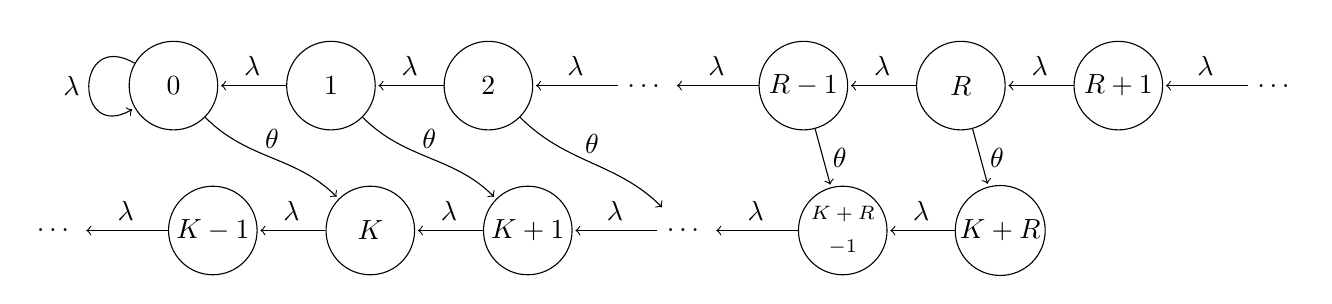
\begin{tikzpicture}[
			node distance={20mm},
			shorten >=1pt,
			main/.style = {draw, circle, minimum size=32pt, inner sep=1pt},
			dots/.style = {minimum size=15pt}
		]
		\node[main] (1) {$0$};
		\node[main] (2) [right of=1] {$1$};
		\node[main] (3) [right of=2] {$2$};
		\node[dots] (d34) [right of=3] {$\dots$};
		\node[main] (4) [right of=d34] {$R-1$};
		\node[main] (5) [right of=4] {$R$};
		\node[main] (6) [right of=5] {$R+1$};
		\node[dots] (d6) [right of=6] {$\dots$};
		\node[dots] (drl) [below=10mm of 1, xshift=-15mm] {$\dots$};
		\node[main] (7) [right of=drl] {$K-1$};
		\node[main] (8) [right of=7] {$K$};
		\node[main] (9) [right of=8] {$K+1$};
		\node[dots] (dkr) [right of=9] {$\dots$};
		\node[main] (10) [right of=dkr] [align=center]{\scriptsize$K+R$ \\ \scriptsize$-1$};
		\node[main] (11) [right of=10] {$K+R$};
		% Draw the lambda edges.
		\draw[->] (1) to [out=150, in=210, looseness=4] node[left] {$\lambda$} (1);
		\draw[->] (2) to node[above] {$\lambda$} (1);
		\draw[->] (3) to node[above] {$\lambda$} (2);
		\draw[->] (d34) to node[above] {$\lambda$} (3);
		\draw[->] (4) to node[above] {$\lambda$} (d34);
		\draw[->] (5) to node[above] {$\lambda$} (4);
		\draw[->] (6) to node[above] {$\lambda$} (5);
		\draw[->] (d6) to node[above] {$\lambda$} (6);
		\draw[->] (7) to node[above] {$\lambda$} (drl);
		\draw[->] (8) to node[above] {$\lambda$} (7);
		\draw[->] (9) to node[above] {$\lambda$} (8);
		\draw[->] (dkr) to node[above] {$\lambda$} (9);
		\draw[->] (10) to node[above] {$\lambda$} (dkr);
		\draw[->] (11) to node[above] {$\lambda$} (10);
		% Draw the theta edges.
		\draw[->] (1) to [out=315, in=135] node[above] {$\theta$} (8);
		\draw[->] (2) to [out=315, in=135] node[above] {$\theta$} (9);
		\draw[->] (3) to [out=315, in=135] node[above] {$\theta$} (dkr);
		\draw[->] (4) to node[right] {$\theta$} (10);
		\draw[->] (5) to node[right] {$\theta$} (11);
	\end{tikzpicture}
\end{center}
Τέλος ο πίνακας ρυθμών μετάβασης είναι ο
\[
	\begin{blockarray}{rcccccccccccc}
		& 0 & 1 & \dots & R-1 & R & \dots & K-1 & K & K+1 & \dots & K+R-1 & K+R \\
		\begin{block}{r(cccccccccccc)}
			0 & \lambda & 0 & \dots & 0 & 0 & \dots & 0 & \theta & 0 & \dots & 0 & 0 \\
			1 & \lambda & 0 & \dots & 0 & 0 & \dots & 0 & 0 & \theta & \dots & 0 & 0 \\
			2 & 0 & \lambda & \dots & 0 & 0 & \dots & 0 & 0 & 0 & \dots & 0 & 0 \\
			\vdots & \vdots & \vdots & \ddots & \vdots & \vdots & \ddots & \vdots & \vdots & \vdots & \ddots & \vdots & \vdots \\
			R-1 & 0 & 0 & \dots & 0 & 0 & \dots & 0 & 0 & 0 & \dots & \theta & 0 \\
			R & 0 & 0 & \dots & \lambda & 0 & \dots & 0 & 0 & 0 & \dots & 0 & \theta \\
			R+1 & 0 & 0 & \dots & 0 & \lambda & \dots & 0 & 0 & 0 & \dots & 0 & 0 \\
			\vdots & \vdots & \vdots & \ddots & \vdots & \vdots & \ddots & \vdots & \vdots & \vdots & \ddots & \vdots & \vdots \\
			K-1 & 0 & 0 & \dots & 0 & 0 & \dots & 0 & 0 & 0 & \dots & 0 & 0 \\
			K & 0 & 0 & \dots & 0 & 0 & \dots & \lambda & 0 & 0 & \dots & 0 & 0 \\
			K+1 & 0 & 0 & \dots & 0 & 0 & \dots & 0 & \lambda & 0 & \dots & 0 & 0 \\
			\vdots & \vdots & \vdots & \ddots & \vdots & \vdots & \ddots & \vdots & \vdots & \vdots & \ddots & \vdots & \vdots \\
			K+R-1 & 0 & 0 & \dots & 0 & 0 & \dots & 0 & 0 & 0 & \dots & 0 & 0 \\
			K+R & 0 & 0 & \dots & 0 & 0 & \dots & 0 & 0 & 0 & \dots & \lambda & 0 \\
		\end{block}
	\end{blockarray}
\]


\section*{Άσκηση 3}

Αρχικά θεωρούμε ότι $Y(t)=0$ για την περίπτωση όπου δεν υπάρχει κανένας πελάτης στο σύστημα και άρα δεν εξυπηρετείται κανένας.
\\[8pt]
Επίσης όταν βρισκόμαστε στην κατάσταση $(0,0)$ τότε για να εξετάσουμε τον τύπο του επόμενου πελάτη που θα φθάσει θεωρούμε την εκλέπτυνση Bernoulli της $\{X(t),t\geq 0\}$ με πιθανότητα επιτυχίας $\alpha$ και $1-\alpha$ αντίστοιχα, οπότε
\begin{itemize}
	\item ρυθμός προσέλευσης πελάτη τύπου $1 \sim \Exp(\alpha \lambda)$
	\item ρυθμός προσέλευσης πελάτη τύπου $2 \sim \Exp((1-\alpha) \lambda)$
\end{itemize}
ενώ από την κατάσταση $(1,1)$ η εξυπηρέτηση του πελάτη γίνεται με ρυθμό $\mu_i$ όπου $i$ ο τύπος του πελάτη.
\\[8pt]
Μετά για $X(t)>1$ έχουμε προσέλευση πελατών με διαδικασία Poisson με παράμετρο $\lambda$ εφόσον μπορούμε να ελέγξουμε για τον τύπο πελάτη όταν φτάσει η στιγμή να εξυπηρετηθεί.
Θεωρούμε λοιπόν ομοίως την εκλέπτυνση Bernoulli της $\{Y(t),t\geq 0\}$ με πιθανότητα επιτυχίας $\alpha$ και $1-\alpha$, οπότε παίρνουμε
\begin{itemize}
	\item ρυθμός εξυπηρέτησης πελάτη τύπου $i$ με τον επόμενο πελάτη να είναι τύπου $1 \sim \Exp(\alpha \mu_i)$
	\item ρυθμός εξυπηρέτησης πελάτη τύπου $i$ με τον επόμενο πελάτη να είναι τύπου $2$\\
		$\sim \Exp((1-\alpha) \mu_i)$
\end{itemize}
Βλέπουμε λοιπόν ότι σε κάθε περίπτωση η μετάβαση από μια κατάσταση σε μια άλλη γίνεται σε χρόνους εκθετικούς και ανεξάρτητους μεταξύ τους και με τις προηγούμενες καταστάσεις, και άρα η $((X(t),Y(t),t\geq 0)$ είναι \mc
\\[8pt]
Ο χώρος καταστάσεων της αλυσίδας είναι $S = \{(0,0)\} \cup \{(i,j)|i=1,2,\dots, j=1,2\}$.
\begin{center}
	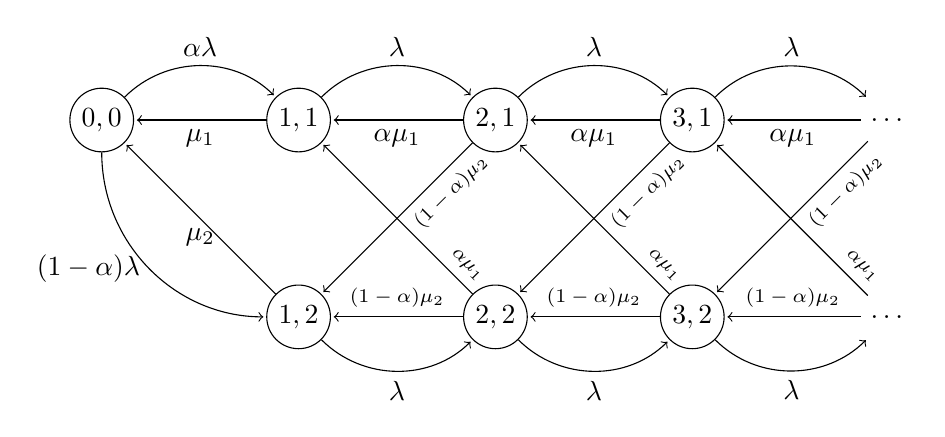
\begin{tikzpicture}[
			node distance={25mm},
			shorten >=1pt,
			main/.style = {draw, circle, minimum size=23pt, inner sep=1pt},
			dots/.style = {minimum size=15pt}
		]
		\node[main] (00) {$0,0$};
		\node[main] (11) [right of=00] {$1,1$};
		\node[main] (21) [right of=11] {$2,1$};
		\node[main] (31) [right of=21] {$3,1$};
		\node[dots] (d1) [right of=31] {$\dots$};
		\node[main] (12) [below of=11] {$1,2$};
		\node[main] (22) [right of=12] {$2,2$};
		\node[main] (32) [right of=22] {$3,2$};
		\node[dots] (d2) [right of=32] {$\dots$};
		% Draw the client type 1 cases.
		\draw[->] (00) to [out=45, in=135] node[above] {$\alpha \lambda$} (11);
		\draw[->] (11) to node[below] {$\mu_1$} (00);
		\draw[->] (11) to [out=45, in=135] node[above] {$\lambda$} (21);
		\draw[->] (21) to node[below] {$\alpha \mu_1$} (11);
		\draw[->] (21) to [out=45, in=135] node[above] {$\lambda$} (31);
		\draw[->] (31) to node[below] {$\alpha \mu_1$} (21);
		\draw[->] (31) to [out=45, in=135] node[above] {$\lambda$} (d1);
		\draw[->] (d1) to node[below] {$\alpha \mu_1$} (31);
		% Draw the client type 2 cases.
		\draw[->] (00) to [out=270, in=180] node[left] {$(1-\alpha) \lambda$} (12);
		\draw[->] (12) to node[below] {$\mu_2$} (00);
		\draw[->] (12) to [out=315, in=225] node[below] {$\lambda$} (22);
		\draw[->] (22) to node[above] {\scriptsize$(1-\alpha) \mu_2$} (12);
		\draw[->] (22) to [out=315, in=225] node[below] {$\lambda$} (32);
		\draw[->] (32) to node[above] {\scriptsize$(1-\alpha) \mu_2$} (22);
		\draw[->] (32) to [out=315, in=225] node[below] {$\lambda$} (d2);
		\draw[->] (d2) to node[above] {\scriptsize$(1-\alpha) \mu_2$} (32);
		% Draw the intersections
		\draw[->] (21) to node[below right, sloped, pos=0.5] {\scriptsize$(1-\alpha) \mu_2$} (12);
		\draw[->] (22) to node[above right, sloped, pos=0.25] {\scriptsize$\alpha \mu_1$} (11);
		\draw[->] (31) to node[below right, sloped, pos=0.5] {\scriptsize$(1-\alpha) \mu_2$} (22);
		\draw[->] (32) to node[above right, sloped, pos=0.25] {\scriptsize$\alpha \mu_1$} (21);
		\draw[->] (d1) to node[below right, sloped, pos=0.5] {\scriptsize$(1-\alpha) \mu_2$} (32);
		\draw[->] (d2) to node[above right, sloped, pos=0.25] {\scriptsize$\alpha \mu_1$} (31);
	\end{tikzpicture}
\end{center}
Τέλος ο πίνακας ρυθμών μετάβασης είναι ο
\[
	\begin{blockarray}{cccccccccc}
		& (0,0) & (1,1) & (2,1) & (3,1) & \dots & (1,2) & (2,2) & (3,2) & \dots \\
		\begin{block}{c(ccccccccc)}
			(0,0) & 0 & \alpha \lambda & 0 & 0 & \dots & (1-\alpha) \lambda & 0 & 0 & \dots \\
			(1,1) & \mu_1 & 0 & \lambda & 0 & \dots & 0 & 0 & 0 & \dots \\
			(2,1) & 0 & \alpha \mu_1 & 0 & \lambda & \dots & (1-\alpha) \mu_2 & 0 & 0 & \dots \\
			(3,1) & 0 & 0 & \alpha \mu_1 & 0 & \dots & 0 & (1-\alpha) \mu_2 & 0 & \dots \\
			\vdots & \vdots & \vdots & \vdots & \vdots & \ddots & \vdots & \vdots & \vdots & \ddots \\
			(1,2) & \mu_2 & 0 & 0 & 0 & \dots & 0 & \lambda & 0 & \dots \\
			(2,2) & 0 & \alpha \mu_1 & 0 & 0 & \dots & (1-\alpha) \mu_2 & 0 & \lambda & \dots \\
			(3,2) & 0 & 0 & \alpha \mu_1 & 0 & \dots & 0 & (1-\alpha) \mu_2 & 0 & \dots \\
			\vdots & \vdots & \vdots & \vdots & \vdots & \ddots & \vdots & \vdots & \vdots & \ddots \\
		\end{block}
	\end{blockarray}
\]


\section*{Άσκηση 4}

Ορίζουμε την αλυσίδα $\{(X(t),Y(t),t\geq 0\}$ όπου η $X(t)$ ο αριθμός των εργασιών που βρίσκονται στον υπολογιστή τη χρονική στιγμή $t$, και $Y(t)=0 \text{ ή } 1$ ανάλογα με το αν ο υπολογιστής είναι λειτουργικός ή όχι τη χρονική στιγμή $t$.
\\[8pt]
Βλέπουμε ότι αν $(X(t),Y(t)) = (i,j)$ για κάποιο $t$ τότε
\begin{itemize}
	\item αν $j=0$ ο υπολογιστής είναι χαλασμένος (και άρα και $i=0$) και είτε θα επισκευαστεί με ρυθμό $b$ είτε θα έρθει μια νέα εργασία με ρυθμό $\lambda$ (η οποία και θα χαθεί αμέσως)
	\item αν $j=1$ τότε ο υπολογιστής είναι λειτουργικός με $i$ εργασίες οπότε
		\begin{itemize}
			\item είτε θα διεκπεραιώσει μια εργασία με ρυθμό $\mu$
			\item είτε θα έρθει νέα εργασία με ρυθμό $\lambda$
			\item είτε θα χαλάσει ο υπολογιστής με ρυθμό $a$
		\end{itemize}
\end{itemize}
Όλες οι διαδικασίες τρέχουν σε εκθετικούς χρόνους ανεξάρτητους μεταξύ τους και από τις προηγούμενες καταστάσεις, και άρα η $\{(X(t),Y(t),t\geq 0\}$ είναι \mc
\\[8pt]
Ο χώρος καταστάσεων της αλυσίδας είναι $S = \{(0,0)\} \cup \{(i,1)|i=0,1,2,\dots\}$.
Για ευκολία στο συμβολισμό θα γράφουμε $-1$ αντί για $(0,0)$ και $i$ αντί για $(i,1)$.
\begin{center}
	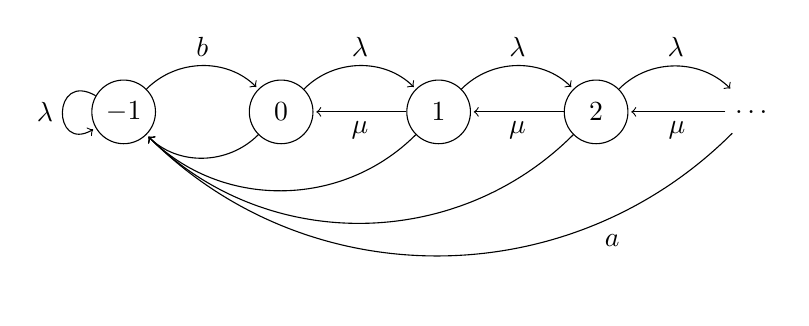
\begin{tikzpicture}[
		node distance={20mm},
		shorten >=1pt,
		main/.style = {draw, circle, minimum size=23pt, inner sep=0pt},
		dots/.style = {minimum size=15pt}
	]
	\node[main] (m1) {$-1$};
	\node[main] (z) [right of=m1] {$0$};
	\node[main] (1) [right of=z] {$1$};
	\node[main] (2) [right of=1] {$2$};
	\node[dots] (d) [right of=2] {$\dots$};
	\draw[->] (m1) to [out=150, in=210, looseness=4] node[left] {$\lambda$} (m1);
	\draw[->] (m1) to [out=45, in=135] node[above] {$b$} (z);
	\draw[->] (z) to [out=225, in=315] (m1);
	\draw[->] (z) to [out=45, in=135] node[above] {$\lambda$} (1);
	\draw[->] (1) to node[below] {$\mu$} (z);
	\draw[->] (1) to [out=225, in=315] (m1);
	\draw[->] (1) to [out=45, in=135] node[above] {$\lambda$} (2);
	\draw[->] (2) to node[below] {$\mu$} (1);
	\draw[->] (2) to [out=225, in=315] (m1);
	\draw[->] (2) to [out=45, in=135] node[above] {$\lambda$} (d);
	\draw[->] (d) to node[below] {$\mu$} (2);
	\draw[->] (d) to [out=225, in=315] node[near start, below right] {$a$} (m1);
	\end{tikzpicture}
\end{center}
Τέλος ο πίνακας ρυθμών μετάβασης είναι ο
\[
	\begin{blockarray}{cccccc}
		& -1 & 0 & 1 & 2 & \dots \\
		\begin{block}{c(ccccc)}
			-1 & \lambda & b & 0 & 0 & \dots \\
			0 & a & 0 & \lambda & 0 & \dots \\
			1 & a & \mu & 0 & \lambda & \dots \\
			2 & a & 0 & \mu & 0 & \dots \\
			\vdots & \vdots & \vdots & \vdots & \vdots & \ddots \\
		\end{block}
	\end{blockarray}
\]
	
\end{document}
